\documentclass[12pt,onecolumn,a4paper]{article}
\usepackage{epsfig,graphicx,subfigure,amsthm,amsmath}
\usepackage{color,xcolor}

\usepackage[margin=1in]{geometry}
\usepackage[numbers]{natbib}

\usepackage{xepersian}
\settextfont[Scale=1.2]{B Nazanin}
\setlatintextfont[Scale=1]{Times New Roman}
\setmathdigitfont{Yas}




\linespread{1.5}


\begin{document}

	\begin{titlepage}
		\begin{center}
			
			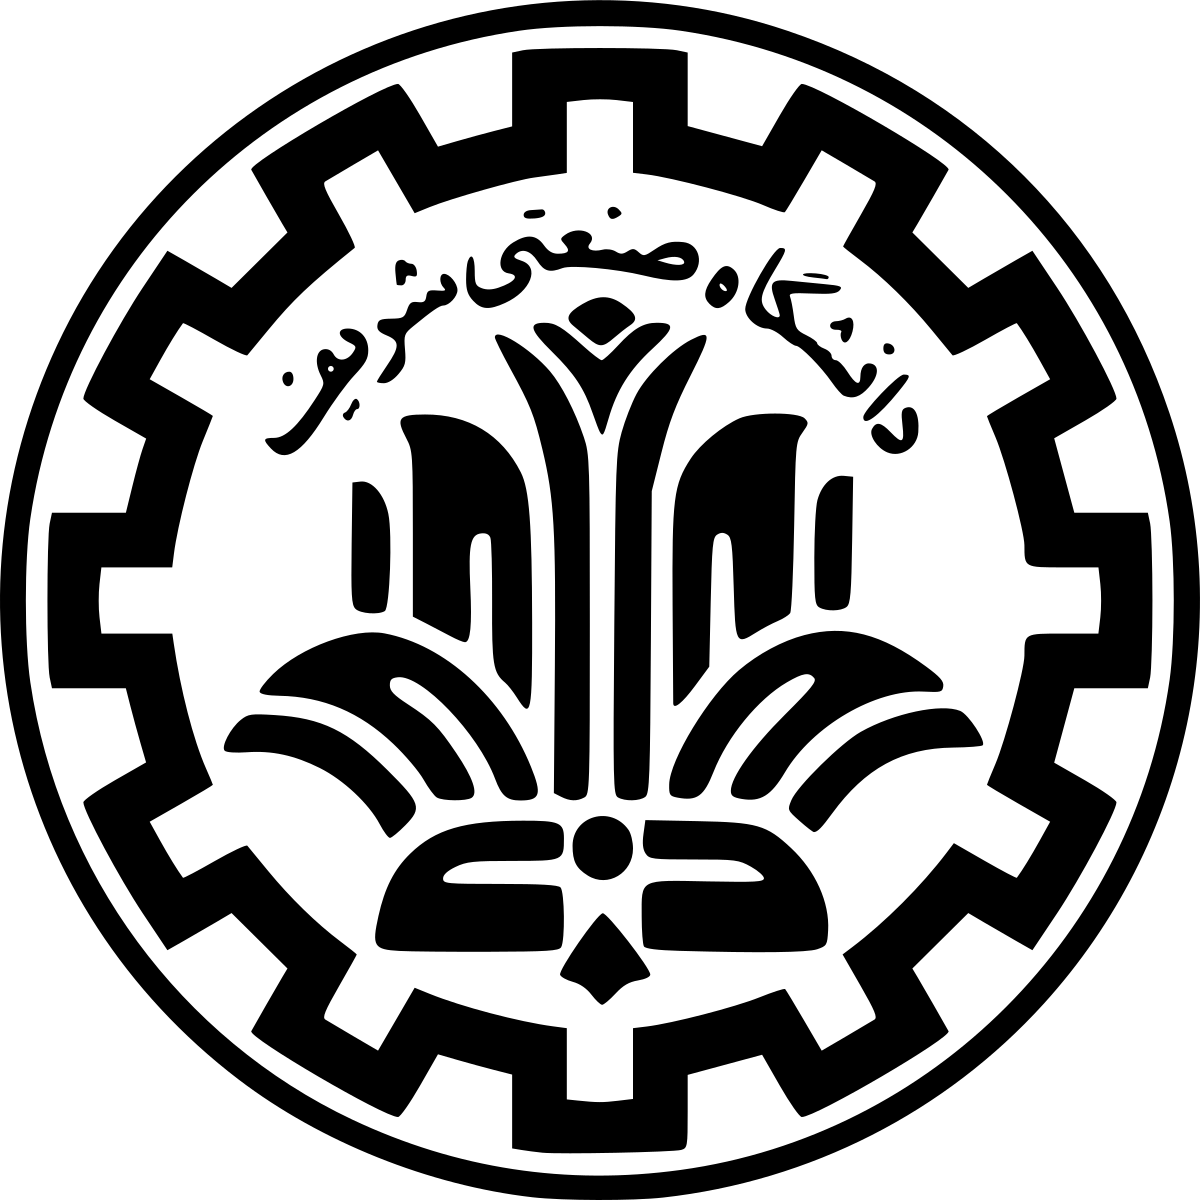
\includegraphics[width=4cm]{assets/logo-sharif.png} % آرم دانشگاه صنعتی شریف
			
			\vspace{1cm}
			
			{\huge \textbf{دانشگاه صنعتی شریف}}  
			
			\vspace{0.5cm}
			
			{\Large دانشکده مهندسی برق}
			
			\vspace{1.5cm}
			
			{\Huge \textbf{گزارش پروژه پایانی}} 
			
			\vspace{0.5cm}
			
			{\Large درس بهینه‌سازی محدب ۲}
			
			\vspace{1.5cm}
			
			{\Huge \textbf{یادگیری گراف با استفاده از همواری}}
			
			\vspace{1.5cm}
			
			\textbf{\Large استاد درس:}  
			
			\vspace{0.5cm}
			
			{\Large دکتر حامد شاه‌منصوری}
			
			\vspace{1.5cm}
			
			\textbf{\Large تهیه‌کنندگان:}  
			
			\vspace{0.5cm}
			
			{\Large محمد رضیئی فیجانی، علی مجلسی}
			
			\vfill
			
			{\Large \today}
			
		\end{center}
	\end{titlepage}
	


    \section{مقدمه}
    
    
    \section{صورت مسئله}
    
    
    
    \bibliographystyle{plainnat-fa}
    \bibliography{assets/references}
	\nocite{*}
\end{document}